\documentclass[12pt]{article}


\usepackage{amssymb}
\usepackage{amsmath}
\usepackage{fullpage}
\usepackage{epsfig}
\usepackage{epstopdf}
\everymath{\displaystyle}



\begin{document}

\begin{center}
\underline{\LARGE{Chapter 1.5 Practice Problems}}
\end{center}

\noindent EXPECTED SKILLS:

\begin{itemize}

\item Know what it means for a function to be continuous at a specific value and on an interval.

\item Find values where a function is not continuous; specifically, you should be able to do this for polynomials, rational functions, exponential and logarithmic functions, and other elementary functions.

\item Determine the values for which a piecewise function is discontinuous, if any such values exist.

\item Use the Intermediate Value Theorem to show the existence of a solution to an equation.

\end{itemize}

\noindent PRACTICE PROBLEMS:

\noindent {\bf Use the graph of $f(x)$, shown below, to answer questions 1-3}

\begin{center}
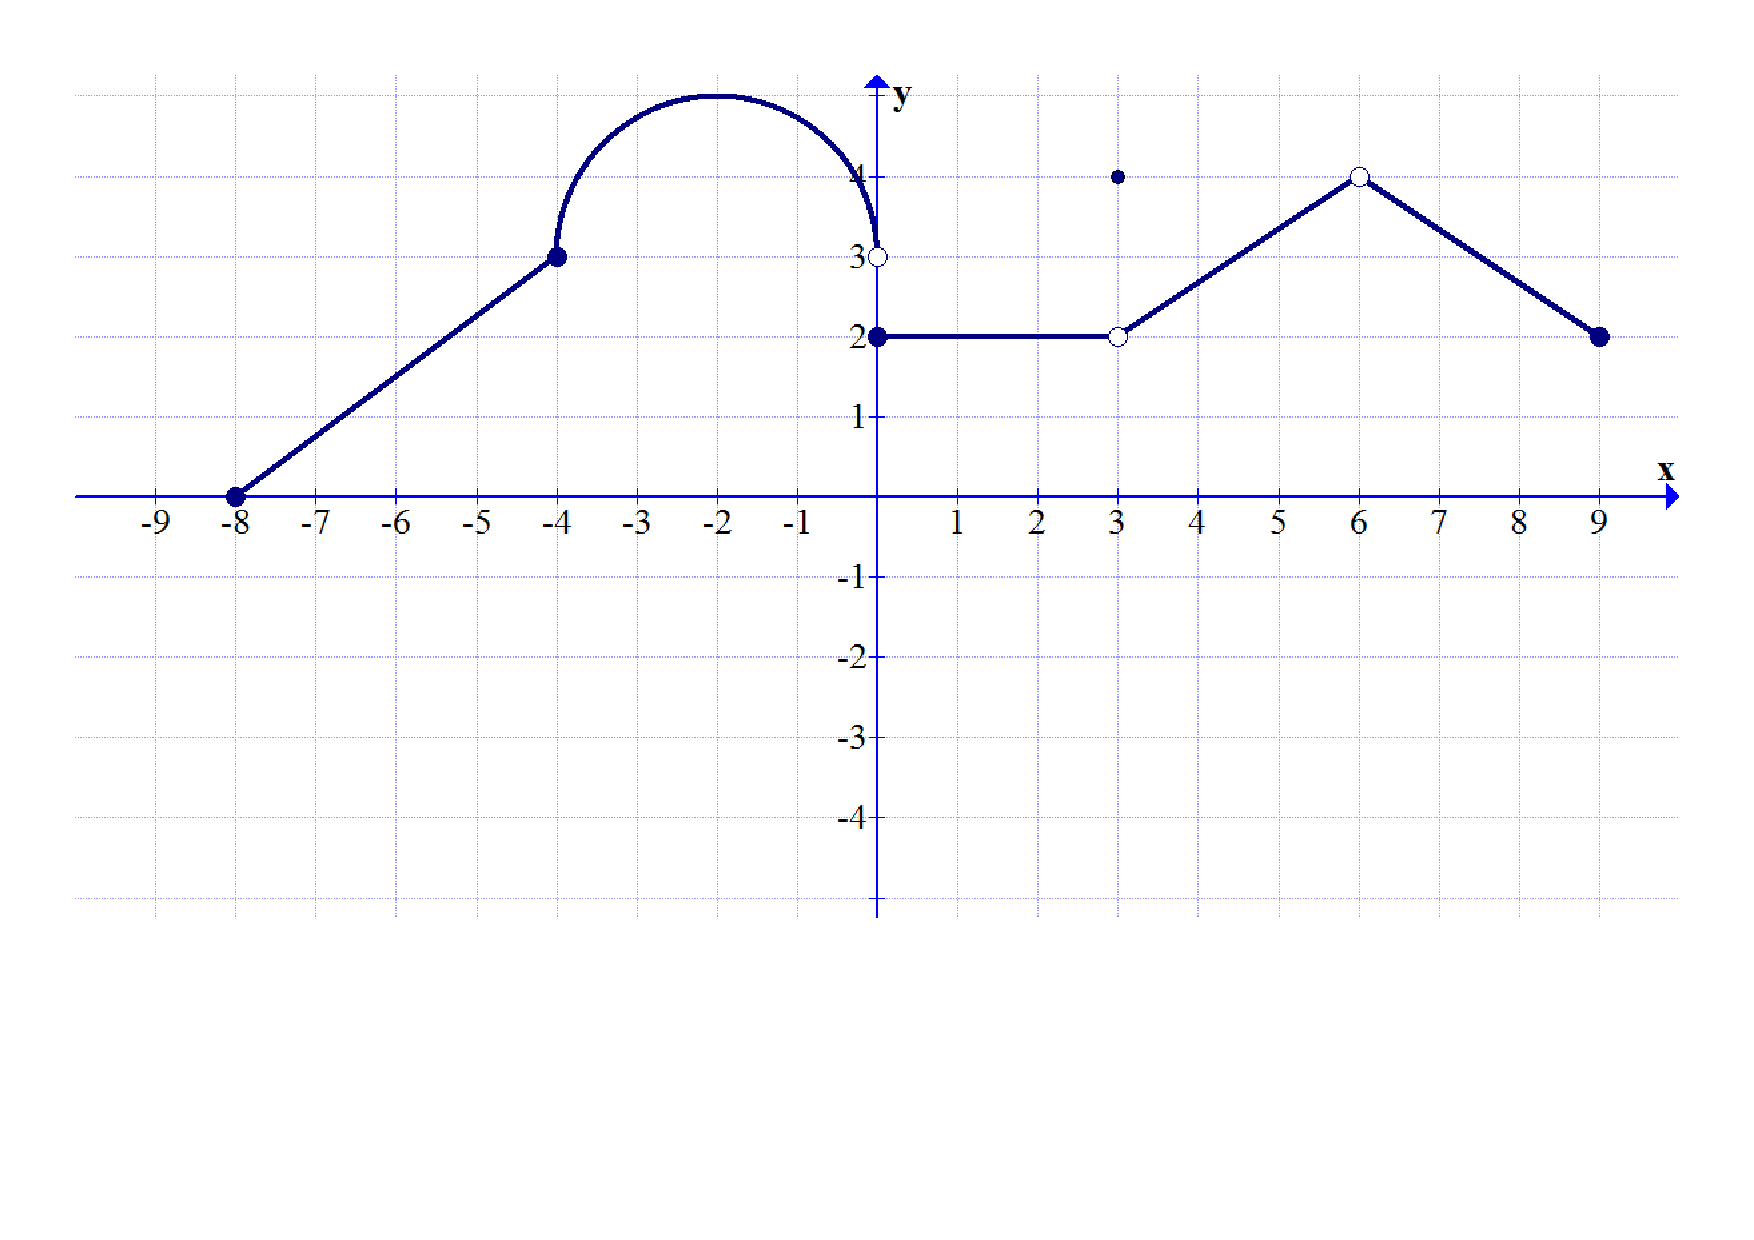
\includegraphics[scale=0.5]{graph.pdf}
\end{center}

\begin{enumerate}

\item For which values of $x$ is $f(x)$ discontinuous?

\includegraphics[scale=0.5]{start.pdf}
{{$f(x)$ is discontinuous when $x=0$, $x=3$, and $x=6$.} }
\includegraphics[scale=0.5]{end.pdf}


\item At each point of discontinuity, explain why $f(x)$ is discontinuous.

\includegraphics[scale=0.5]{start.pdf}
{{\begin{tabular}{l}
At $x=0$, $f(x)$ is discontinuous because $\displaystyle \lim_{x \rightarrow 0}{f(x)}$ DNE.\\
At $x=3$, $f(x)$ is discontinuous because $\displaystyle \lim_{x \rightarrow 3}{f(x)} \neq f(3)$.\\
At $x=6$, $f(x)$ is discontinuous because $f(6)$ is undefined
\end{tabular}}}
\includegraphics[scale=0.5]{end.pdf}


\item Determine whether $f(x)$ is continuous on the given interval.  If not, explain why.

\begin{enumerate}

\item $[-8,-4]$

\includegraphics[scale=0.5]{start.pdf}
{{Yes}}
\includegraphics[scale=0.5]{end.pdf}


\item $[-8,0]$

\includegraphics[scale=0.5]{start.pdf}
{{No because $\displaystyle \lim_{x \rightarrow 0^-}{f(x)} \neq f(0)$}}
\includegraphics[scale=0.5]{end.pdf}


\item $[-8,0)$

\includegraphics[scale=0.5]{start.pdf}
{{Yes}}
\includegraphics[scale=0.5]{end.pdf}


\item $[-2,1]$

\includegraphics[scale=0.5]{start.pdf}
{{No because $\displaystyle \lim_{x\rightarrow 0}{f(x)}$ DNE}}
\includegraphics[scale=0.5]{end.pdf}


\item $(3,6)$

\includegraphics[scale=0.5]{start.pdf}
{{Yes}}
\includegraphics[scale=0.5]{end.pdf}


\item $[3,6)$

\includegraphics[scale=0.5]{start.pdf}
{{No because $\displaystyle \lim_{x\rightarrow 3^+}{f(x)} \neq f(3)$}}
\includegraphics[scale=0.5]{end.pdf}


\item $(6,9]$

\includegraphics[scale=0.5]{start.pdf}
{{Yes}}
\includegraphics[scale=0.5]{end.pdf}


\item $[6,9]$

\includegraphics[scale=0.5]{start.pdf}
{{No because $f(6)$ is undefined}}
\includegraphics[scale=0.5]{end.pdf}


\end{enumerate}

\item For each of the following, sketch the graph of a function, $y=f(x)$, which satisfies the given characteristic.  (There are many possible answers for each)

\begin{enumerate}

\item $f(x)$ is continuous everywhere except at $x=1$.

\includegraphics[scale=0.5]{start.pdf}
{{{1\linewidth}{Any graph for which either $f(1)$ is undefined or $\displaystyle \lim_{x \rightarrow 1}{f(x)}$ DNE or $\displaystyle \lim_{x \rightarrow 1}{f(x)} \neq f(1)$}}}
\includegraphics[scale=0.5]{end.pdf}


\item $f(x)$ is continuous everywhere except at $x=-2$ where the $\displaystyle \lim_{x \rightarrow -2^-}{f(x)}=\lim_{x \rightarrow -2^+}{f(x)}$.

\includegraphics[scale=0.5]{start.pdf}
{{Any graph for which either $f(-2)$ is undefined or $\displaystyle \lim_{x \rightarrow -2}{f(x)} \neq f(-2)$}}
\includegraphics[scale=0.5]{end.pdf}


\item $f(x)$ is continuous everywhere except at $x=0$, where $f(0)=2$.

\includegraphics[scale=0.5]{start.pdf}
{{Any graph for which $\displaystyle \lim_{x \rightarrow 0}{f(x)}$ DNE or $\displaystyle \lim_{x \rightarrow 0}{f(x)} \neq 2$}}
\includegraphics[scale=0.5]{end.pdf}


\end{enumerate}

\item Sketch the graph of a function which satisfies the following criteria:

\begin{itemize}

\item The domain of $f(x)$ is $[1,3]$

\item $f(x)$ is continuous on $[1,2]$ and $(2,3]$.

\item $f(x)$ is not continuous on $[1,3]$

\end{itemize}

\includegraphics[scale=0.5]{start.pdf}
{{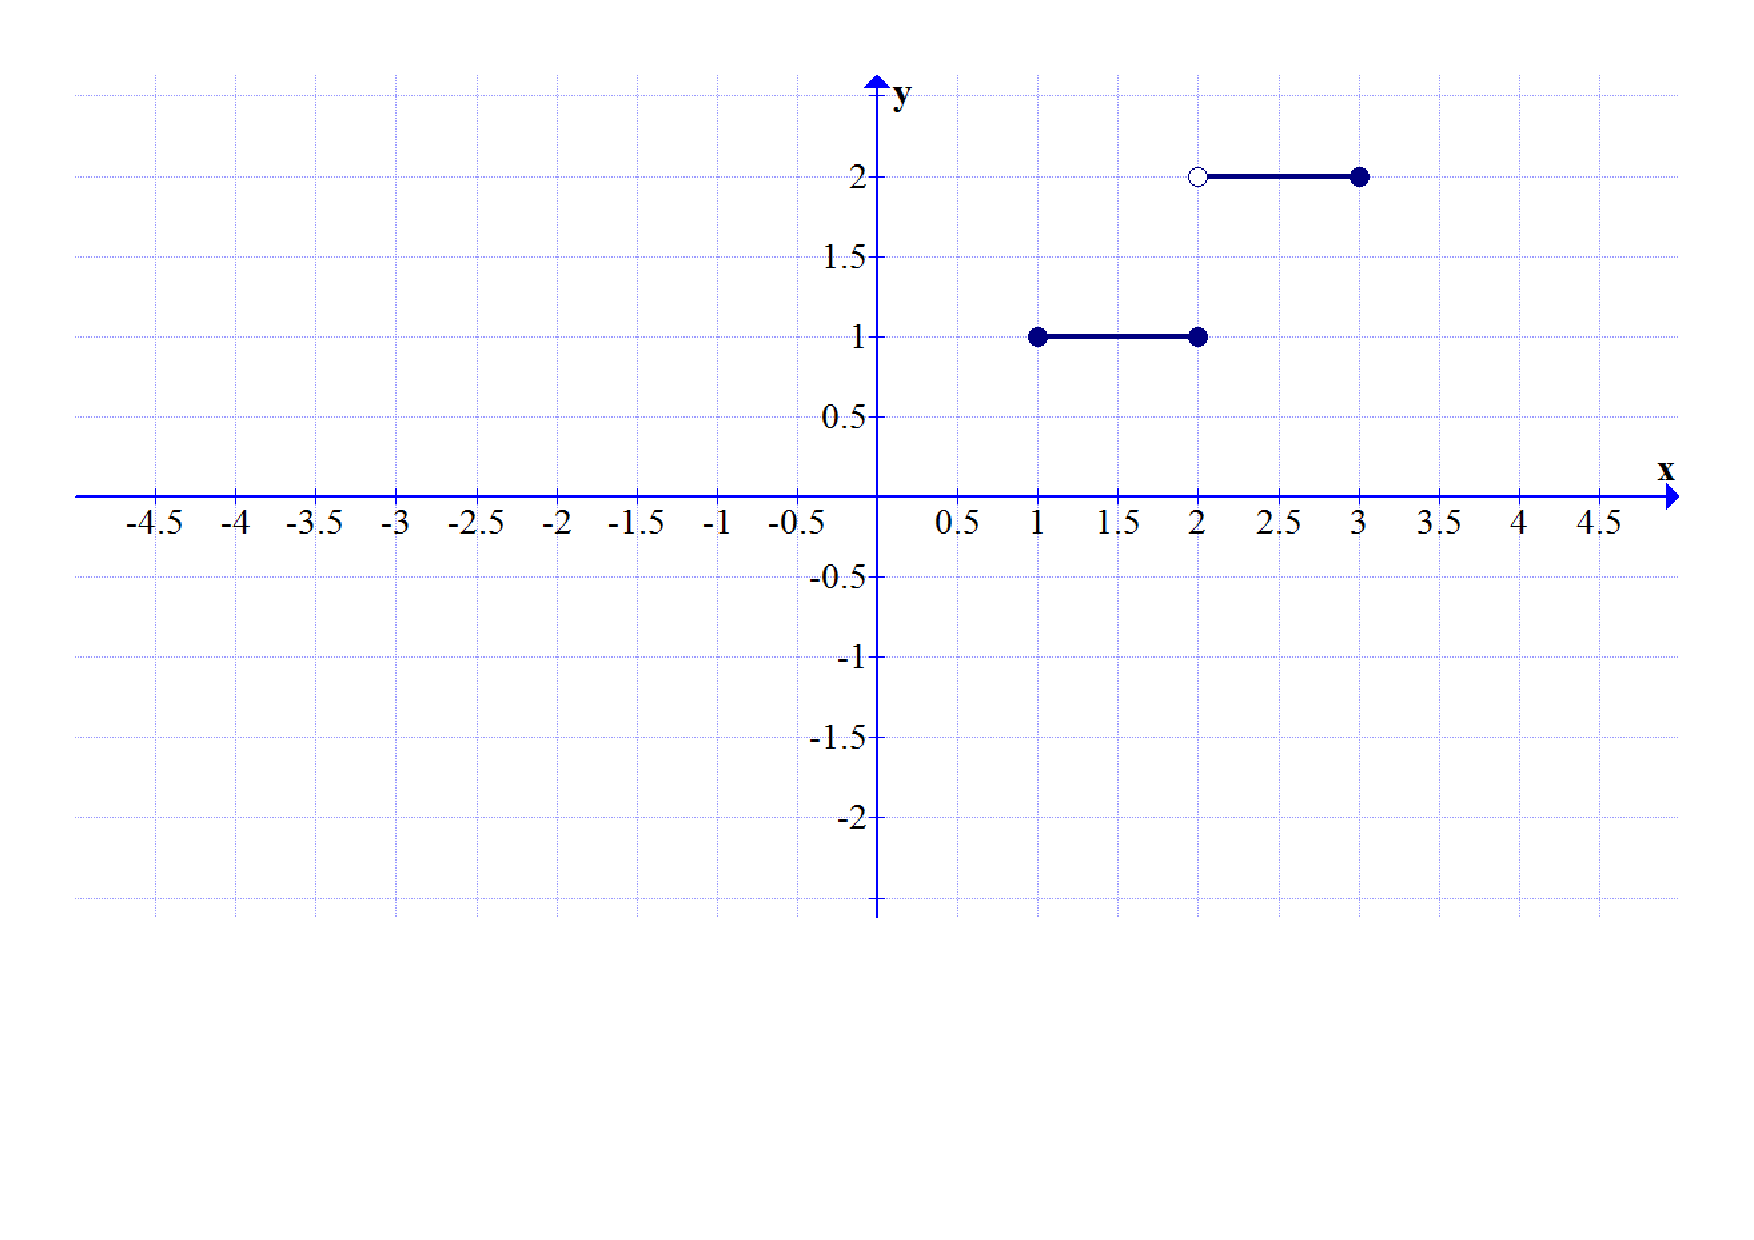
\includegraphics[scale=0.5]{graph1.pdf}}}
\includegraphics[scale=0.5]{end.pdf}


\end{enumerate}

\noindent {\bf For problems 6-15, determine the value(s) of $x$ where the given function has a point of discontinuity, if any such values exist.}

\begin{enumerate}
\setcounter{enumi}{5}

\item $f(x) = |x|$ 

\includegraphics[scale=0.5]{start.pdf}
{{$f(x)$ is always continuous}}
\includegraphics[scale=0.5]{end.pdf}


\item $f(x) = x^2 -x -5$

\includegraphics[scale=0.5]{start.pdf}
{{$f(x)$ is always continuous}}
\includegraphics[scale=0.5]{end.pdf}


\item $f(x) = \frac{x}{x-1}$ 

\includegraphics[scale=0.5]{start.pdf}
{{$f(x)$ has a discontinuity when $x=1$}}
\includegraphics[scale=0.5]{end.pdf}


\item $f(x) = \sqrt[3]{x-1}$ 

\includegraphics[scale=0.5]{start.pdf}
{{$f(x)$  is always continuous}}
\includegraphics[scale=0.5]{end.pdf}


\item $f(x) = \frac{x^2+3x-10}{x-7}$ 

\includegraphics[scale=0.5]{start.pdf}
{{$f(x)$ has discontinuity when $x=7$}}
\includegraphics[scale=0.5]{end.pdf}


\item $f(x) = \frac{x^2-4}{x-2}$ 

\includegraphics[scale=0.5]{start.pdf}
{{$f(x)$ has a discontinuity when $x=2$}}
\includegraphics[scale=0.5]{end.pdf}


\item$f(x) = \frac{1}{x^2-2}+\frac{x^3-1}{2x^2-1}$ 

\includegraphics[scale=0.5]{start.pdf}
{{$f(x)$ has a discontinuity when $x=\sqrt{2}$, $x=-\sqrt{2}$, $\displaystyle x=\frac{\sqrt{2}}{2}$, and $\displaystyle x=-\frac{\sqrt{2}}{2}$}}
\includegraphics[scale=0.5]{end.pdf}


\item $f(x) = \begin{cases} 
x^2-1, & \text{if } x<2 \\
\frac{3}{x-1}, & \text{if } x\geq 2\end{cases}$ 

\includegraphics[scale=0.5]{start.pdf}
{{$f(x)$ is always continuous}}
\includegraphics[scale=0.5]{end.pdf}


\item $f(x) = \begin{cases} 
5+\frac{1}{x}, & \text{if } x<- 1 \\
3x^2+2x+3, & \text{if } x> -1\end{cases} $ 

\includegraphics[scale=0.5]{start.pdf}
{{$f(x)$ has a discontinuity when $x=-1$}}
\includegraphics[scale=0.5]{end.pdf}


\item $f(x) = \begin{cases} 
x^2-3x+4, & \text{if } x\leq1 \\
x^4-4x^3-2x^2+6, & \text{if } x>1 \end{cases}$ 

\includegraphics[scale=0.5]{start.pdf}
{{$f(x)$ has discontinuity when $x=1$}}
\includegraphics[scale=0.5]{end.pdf}


\item Find the value(s) of $k$ such that $f(x)$ is continuous everywhere:\\
$$\displaystyle f(x) = \begin{cases}
x^2-7, & \text{if } x\leq 2 \\
4x^3-3kx+2, & \text{if } x>2 \end{cases}$$

\includegraphics[scale=0.5]{start.pdf}
{{$\displaystyle k=\frac{37}{6}$}}
\includegraphics[scale=0.5]{end.pdf}


\item Find the value(s) of $k$ and $m$ such that $f(x)$ is continuous everywhere: $$f(x) = \begin{cases}
2x+8m, & \text{if } x\leq -2 \\
mx+k, & \text{if } -2<x \leq 2 \\
-3x^2+8x-2k, & \text{if } x>2 \end{cases}$$ 

\includegraphics[scale=0.5]{start.pdf}
{{$\displaystyle m = \frac{1}{2}$ and $k=1$}}
\includegraphics[scale=0.5]{end.pdf}


\item {\bf Multiple Choice:} Where is $f(x)=\frac{\sqrt{x-2}}{x^2-x}$ continuous?

\begin{enumerate}

\item $x\neq 0$ and $x \neq 1$

\item $x \leq 2$ where $x\neq 0$ and $x \neq 1$

\item $x\leq 2$

\item $x \geq 2$

\item $|x|>2$

\end{enumerate}

\includegraphics[scale=0.5]{start.pdf}
{{d}}
\includegraphics[scale=0.5]{end.pdf}


\item Consider the following definitions:

\begin{itemize}

\item {\bf Definition:} A function $f(x)$ has a \underline{removable discontinuity} at $x=a$ if $\displaystyle \lim_{x\rightarrow a}{f(x)}$ exists but $f(x)$ is not continuous at $x=a$.  This could be because $f(a)$ is undefined or because $\displaystyle \lim_{x\rightarrow a}{f(x)} \neq f(a)$.

\item {\bf Definition:} A function $f(x)$ has a \underline{jump discontinuity} at $x=a$ if $\displaystyle \lim_{x \rightarrow a^-}{f(x)}$ exists and $\displaystyle \lim_{x \rightarrow a^+}{f(x)}$ exists, but $\displaystyle \lim_{x \rightarrow a^-}{f(x)}\neq \lim_{x \rightarrow a^+}{f(x)}$

\end{itemize}

For each of the follwing, determine the value(s) of $x$ where the given function has a point of discontinuity.  Classify each discontinuity as a removable discontinuity, a jump discontinuity, or neither.

\begin{enumerate}

\item $f(x)=\frac{x^2-4}{x-2}$

\includegraphics[scale=0.5]{start.pdf}
{{$f(x)$ has a removable discontinuity when $x=2$}}
\includegraphics[scale=0.5]{end.pdf}


\item $f(x)=\frac{x-1}{x-4}$

\includegraphics[scale=0.5]{start.pdf}
{{{1\linewidth}{$f(x)$ has a discontinuity when $x=4$; it is neither a removable discontinuity nor a jump discontinuity.}}}
\includegraphics[scale=0.5]{end.pdf}


\item $f(x) = \begin{cases} 
x^2-3x+4, & \text{if } x\leq1 \\
x^4-4x^3-2x^2+6, & \text{if } x>1 \end{cases}$ 

\includegraphics[scale=0.5]{start.pdf}
{{$f(x)$ has jump discontinuity when $x=1$}}
\includegraphics[scale=0.5]{end.pdf}


\item $f(x)=\frac{x-1}{x^2-4x+3}$

\includegraphics[scale=0.5]{start.pdf}
{{{1\linewidth}{$f(x)$ has a removable discontinuity when $x=1$.  $f(x)$ has another discontinuity when $x=3$; it is neither a removable discontinuity nor a jump discontinuity.}}}
\includegraphics[scale=0.5]{end.pdf}


\end{enumerate}

\item {\bf Multiple Choice:} Consider the function:$$f(x)=\begin{cases}
x^2 & \text{if }  x<-2\\
4 & \text{if }  -2<x\leq 1\\
6-x & \text{if }  x>1 \end{cases}$$  Which of the following statements is true about $f(x)$?

\begin{enumerate}

\item $f(x)$ is continuous everywhere.

\item If $f(-2)$ were defined to be 4, then $f(x)$ would be continuous everywhere.

\item The only discontinuity of $f(x)$ occurs when $x=-2$.

\item The only discontinuity of $f(x)$ occurs when $x=1$.

\item The only discontinuities of $f(x)$ occur when $x=-2$ and $x=1$.

\end{enumerate}

\includegraphics[scale=0.5]{start.pdf}
{{e}}
\includegraphics[scale=0.5]{end.pdf}


\item Show that the equation $x^3-x^2+3x-1=1$ has at least one solution in $(0,1)$. 

\includegraphics[scale=0.5]{start.pdf}
{{{1\linewidth}{Let $f(x) = x^3-x^2+3x-2$. It suffices to show that there exists a $c$ in $(0,1)$ such that $f(c)=0$.  Since $f(x)$ is a polynomial, it is continuous everywhere on $(-\infty,\infty)$.  Specifically, it is continuous on $[0,1]$.  Since $f(0)=-2<0$ and $f(1)=1>0$, the Intermediate Value Theorem states that there exists some $c in (0,1)$, $f(c)=0$.  The result follows.}}}
\includegraphics[scale=0.5]{end.pdf}


\item Show that $f(x)=x^3-9x+5$ has at least one $x$-intercept in $(1,10)$.

\includegraphics[scale=0.5]{start.pdf}
{{{1\linewidth}{We need to show that there exists at least one solution to $f(x)=0$.  Since $f(x)$ is a polynomial, it is continuous on $[1,10]$.  Notice that $f(1)=-3<0$ and $f(10)=915>0$.  Thus, the Intermediate Value Theorem states that there must be a $c$ in $(1,10)$ with $f(c)=0$.}}}
\includegraphics[scale=0.5]{end.pdf}


\item Use the intermediate value theorem to show that $x^3-2x^2-2x+1=0$ has at least {\bf TWO} solutions in $[0,5]$.

\includegraphics[scale=0.5]{start.pdf}
{{{1\linewidth}{We will apply the IVT twice -- first on $[0,1]$ and then on $[1,5]$.  Let $f(x)=x^3-2x^2-2x+1$.  Since $f(x)$ is a polynomial, it is continuous on $(-\infty,\infty)$.  As a result, it is continuous on $[0,1]$ and $[1,5]$.  Notice that $f(0)=1>0$ and $f(1)=-2<0$.  So, the IVT implies that there exists a $c$ in $(0,1)$ such that $f(c)=0$.  Similarly, notice that $f(1)=-2<0$ and $f(5)=66>0$.  So, the IVT implies that there exists a $d$ in $(1,5)$ such that $f(d)=0$.}}}
\includegraphics[scale=0.5]{end.pdf}


\end{enumerate}

\end{document}